\documentclass[12pt, titlepage]{article}

\usepackage{graphicx}
\usepackage{float}
\usepackage{booktabs}
\usepackage{tabularx}
\usepackage{hyperref}
\hypersetup{
    colorlinks,
    citecolor=black,
    filecolor=black,
    linkcolor=red,
    urlcolor=blue
}
\usepackage[round]{natbib}



\begin{document}

\title{Usability Report: Software Engineering} 
\author{Team \#11, OKKM Insights\\
Mathew Petronilho\\
Oleg Glotov\\
Kyle McMaster\\
Kartik Chaudhari}
\date{\today}
	
\maketitle

\pagenumbering{roman}

\section{Revision History}

\begin{tabularx}{\textwidth}{p{3cm}p{2cm}X}
\toprule {\bf Date} & {\bf Version} & {\bf Notes}\\
\midrule
10/03/2025 & 1.0  &\\
03/04/2025 & 2.0  &\\
\bottomrule
\end{tabularx}


\tableofcontents

\pagenumbering{arabic}
\section{Preliminary Survey}
As a first look into the usability of OrbitWatch, we have conducted a preliminary survey of potential users. The objective of this test is to determine areas for improvement between the Rev0 version of the website and Rev1.
\subsection{Materials}
The following survey was presented to five usability testers. 
\begin{centering}
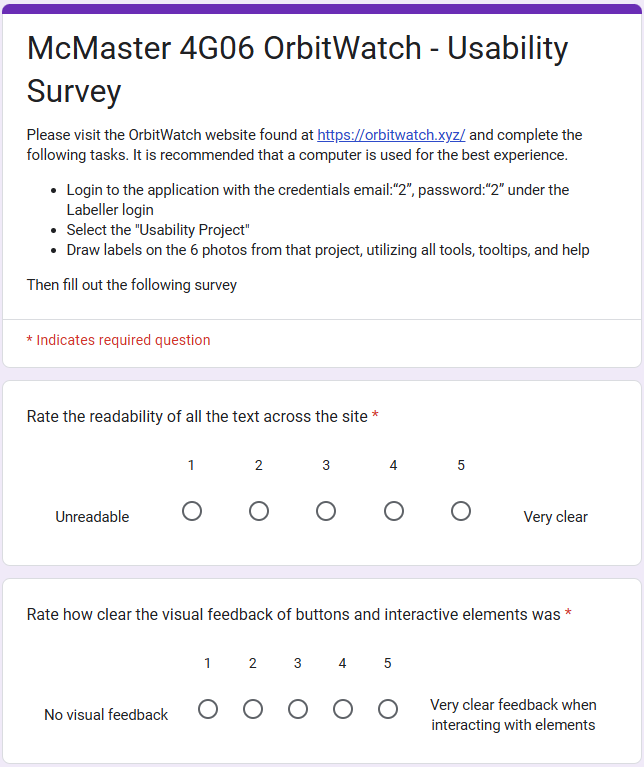
\includegraphics[scale=0.7]{Survey (3).png}\\
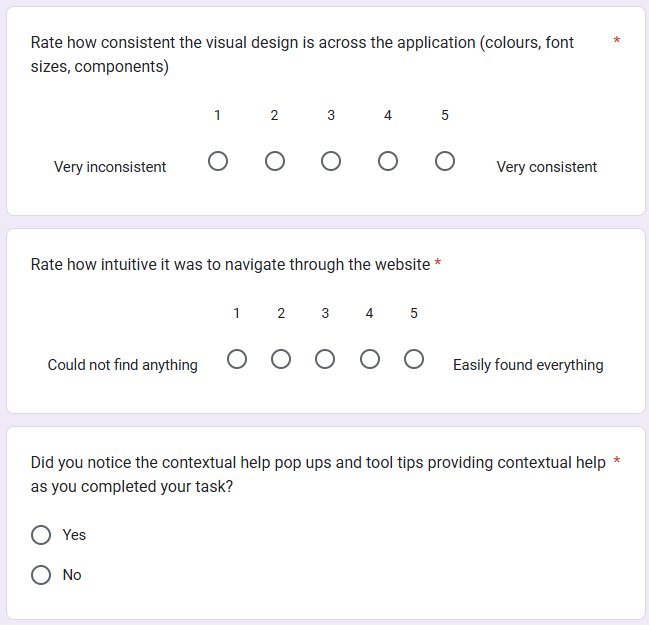
\includegraphics[scale=0.7]{Survey (4).png}\\
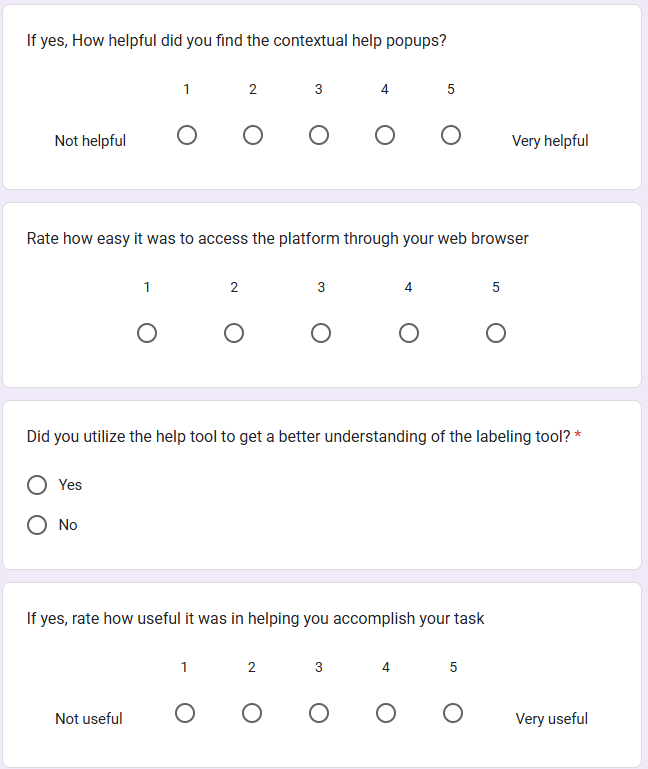
\includegraphics[scale=0.7]{Survey (1).png}\\
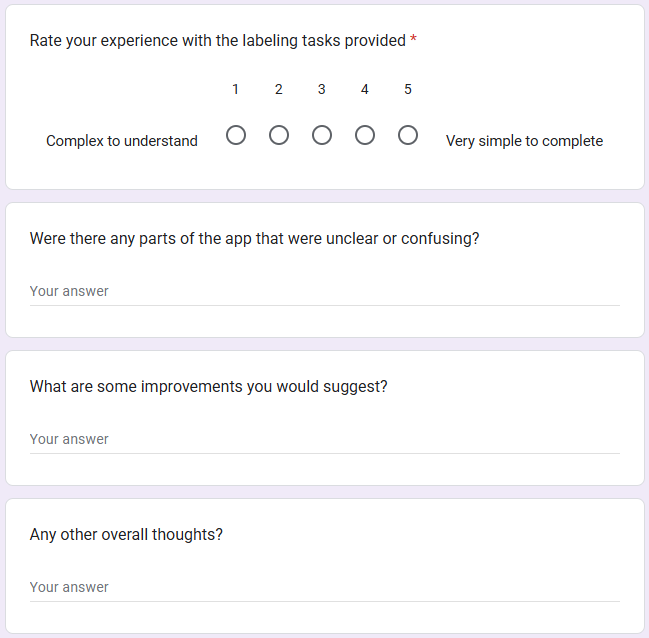
\includegraphics[scale=0.7]{Survey (2).png}\\
\end{centering}
Each of the testers is aged 20-26, university educated, and familiar with technology. We understand this to be a limitation of our experiment, as ideally we would have access to testers from a wider range of ages, backgrounds, and expertise. However, we believe the result from this 
survey remain valuable to identify areas for improvement for our website's usability.
\subsection{Results}
After conducting the survey, we have received the following results.
\begin{centering}
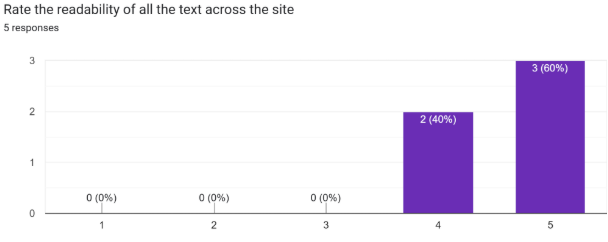
\includegraphics[scale=0.7]{chart (2).png}\\
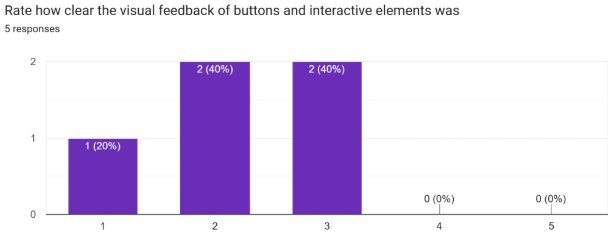
\includegraphics[scale=0.7]{chart (3).png}\\
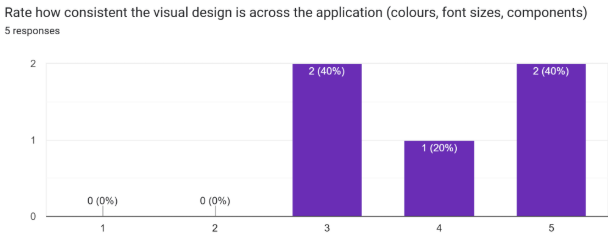
\includegraphics[scale=0.7]{chart (4).png}\\
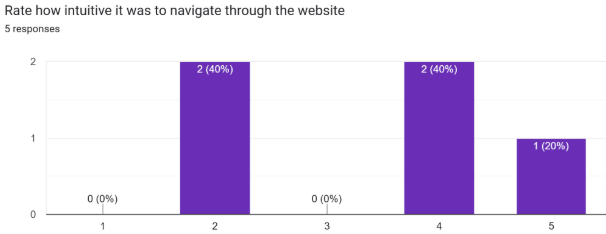
\includegraphics[scale=0.7]{chart (5).png}\\
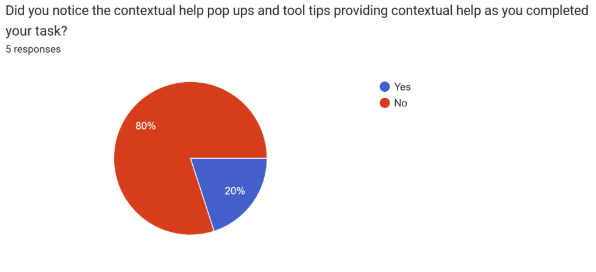
\includegraphics[scale=0.7]{chart (6).png}\\
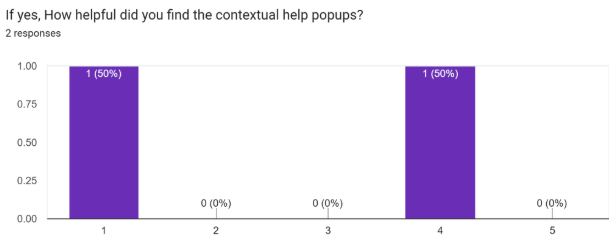
\includegraphics[scale=0.7]{chart (7).png}\\
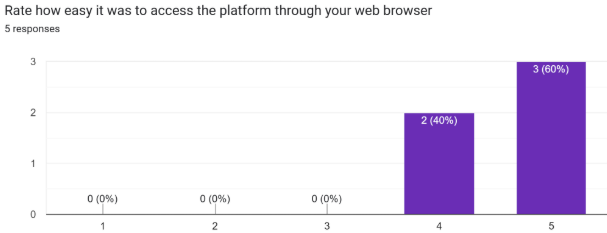
\includegraphics[scale=0.7]{chart (8).png}\\
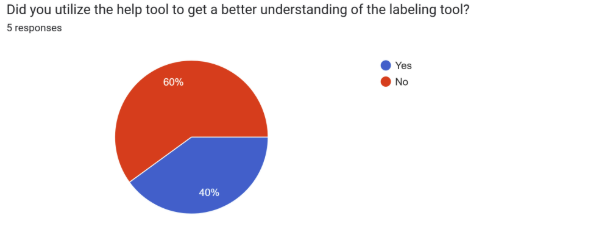
\includegraphics[scale=0.7]{chart (9).png}\\
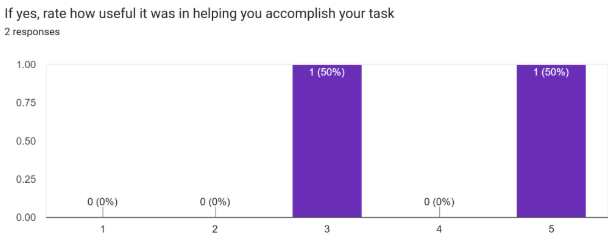
\includegraphics[scale=0.7]{chart (10).png}\\
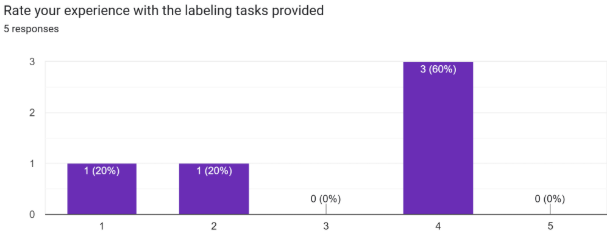
\includegraphics[scale=0.7]{chart (1).png}\\
\end{centering}
We also obtained qualitative feedback, which will be discussed in the analysis section.
\subsection{Analysis}
From these results, some obvious trends emerge. First, readability and design are the current strong points. Most people agree that the text is readable, and the design is consistent. This is critical for improving the discoverability of the site.
Unfortunately, there are quite a few more areas for improvement. Several of the respondents reported that it was challenging to know what to do. They were unaware of the purpose of the website and of the features available to them. One user commented `The overall concept of the application was slightly confusing, the help button did aid in learning what to do. I thought I was only allowed to label once, before realizing I have to select the same label button multiple times.'
It is very important that we ensure new users are able to complete tasks easily. Otherwise, we may lose users to frustration. One user suggested including a `3-second gif' of someone labeling a similar image before a user labels for the first time. This would likely be enough to eliminate a lot of confusion from the users. Another area for improvement is related to feedback when labelling. Several users were unsure when a label was submitted, or what buttons like `skip' or `next' do. 
This will again lead to frustration and confusion, alienating users. 

\subsection{Next Steps}
We will implement the feedback collected in this first survey to improve the site for Rev1. After changes have been implemented, we will redistribute the survey to the same testers. We are hoping to see an improvement in the rating collected between the first and second survey.


\section{Follow-up Survey}
After making improvements to the user interface, we were interested to see if the changes satisfactorily addressed the concerns from the original design. 
We are very proud to report that there was a significant improvement in our usability metrics. This section will describe the materials, results, and analysis of the follow-up survey.

\subsection{Materials}
A copy of the original survey was resent to the same usability testers. This was done to understand the relative improvement over original scores, instead of introducing
potential variability in `user-rating baselines'. By using the same people, we can more accurately conclude if the UI improved, instead of if the new set of participants rates things more highly on average.
\subsection{Results}
In the follow-up survey, we obtained the following results:

\begin{centering}
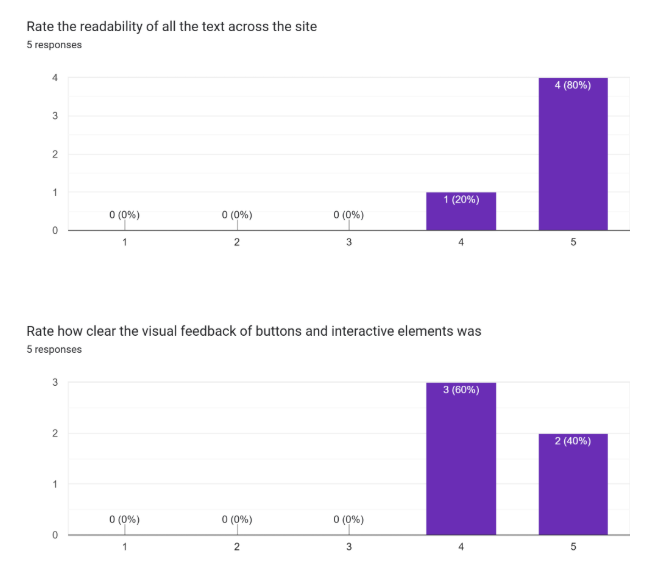
\includegraphics[scale=0.7]{chart_2_1.png}\\
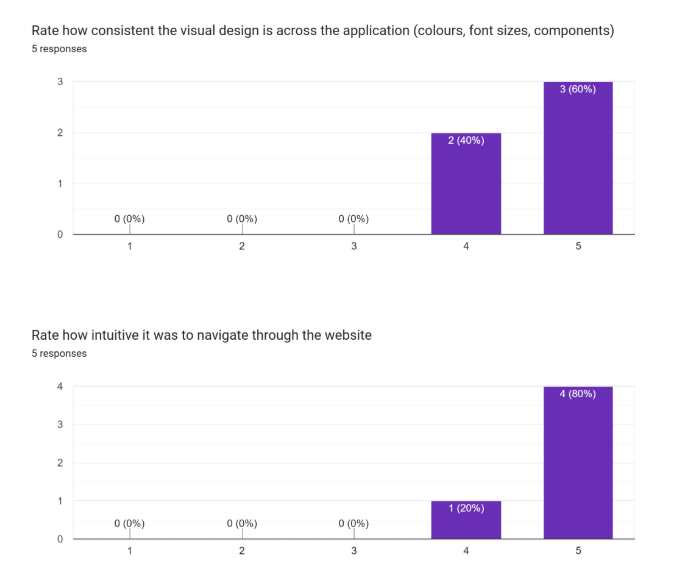
\includegraphics[scale=0.7]{chart_2_2.png}\\
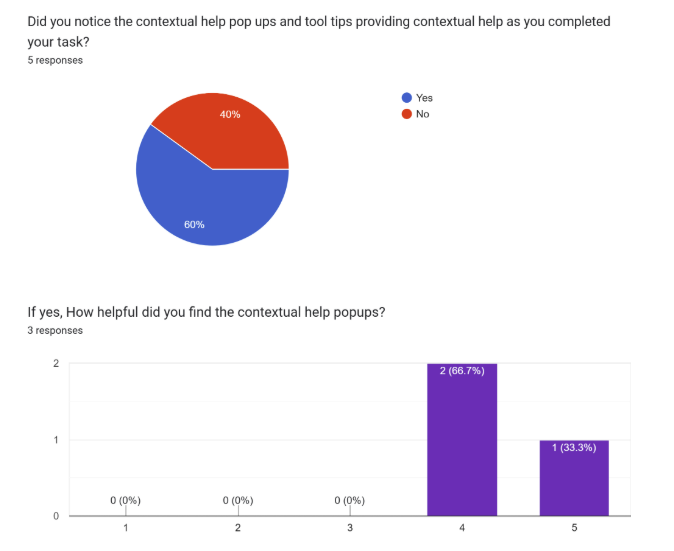
\includegraphics[scale=0.7]{chart_2_3.png}\\
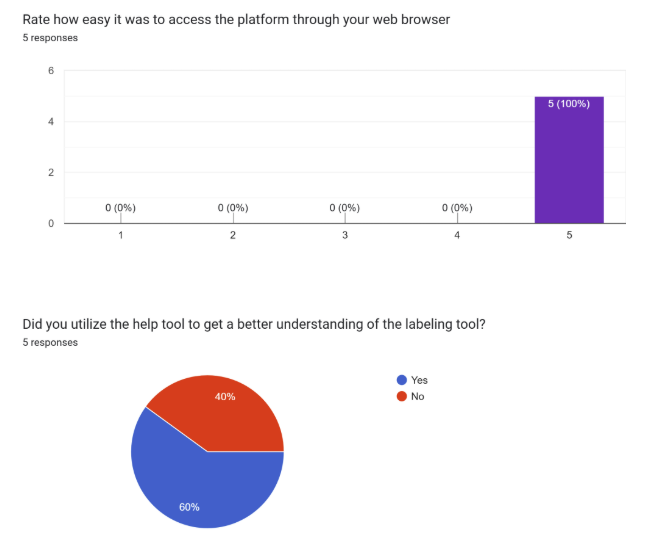
\includegraphics[scale=0.7]{chart_2_4.png}\\
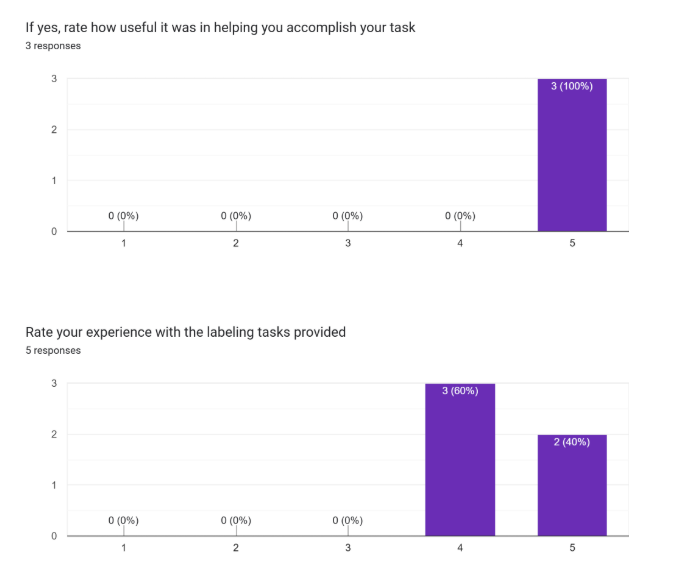
\includegraphics[scale=0.7]{chart_2_5.png}\\
\end{centering}

Again, the qualitative results will be discussed in the analysis section.

\subsection{Analysis}
These results provide strong evidence that the changes made to the front end improved the usability of the website. In each survey question, the average score increased.
One area of focus was on the labelling experience. In contrast to the first iteration, each tester reported a positive experience with the labelling tasks. This is likely attributed to the 
new, in-house labelling library we developed to address user concerns. One tester commented that ``It is much easier to draw multiple labels now. I don't have to reselect the box each time anymore''.
We also noticed an improvement in our help tools. On the last survey, two testers used the help tool, and reported an average score of 4/5. In the new design, the help tool was used 3 times with everyone reporting its usefulness to be 5/5.
In the redesign, we made the help tool more apparent, and made the features it contains more useful. In the last survey, a tester recommended we include a short gif of someone completing a labelling task at the start of the help screen. This, among other changes, are likely the reason for the improved score.


One limitation of the study to consider is that each of the testers have had one prior experience with the tool before completing the second survey. This means that they have some knowledge of what to expect, and therefore certain results should not be expected to translate to new users. 
For example, we would expect the navigation scores to increase, even without changes to the UI as testers become more familiar with the task at hand. In the future, similar studies should be done on a larger pool of first-time users to the site.




\end{document}
